\newpage
\section{Backtracking}
\subsection{Rationale of the Backtracking Algorithms}

The basic idea is that suppose we have a partial solution $( x_1, \dots , x_i )$ where each $x_k \in S_k$ for  $1 \le k \le i < n$.   First we add  $x_{i+1} \in S_{i+1}$ and check if $( x_1, \dots , x_i, x_{i+1} )$ satisfies the constrains.  If the answer is ``yes'' we continue to add the next $x$, else we delete $x_i$ and backtrack to the previous partial solution $( x_1, \dots , x_{i-1} )$.

先决策点少的状态. 

\subsection{The Turnpike Reconstruction Problem}
Given $N$ points on the $x$-axis with coordinates $x_1 <  x_2 < \dots < x_N$ .  Assume that $x_1 = 0$.  There are $N ( N – 1 ) / 2$ distances between every pair of points. Given $N ( N – 1 ) / 2$ distances.  Reconstruct a point set from the distances. 

手玩使用性质搜索


\subsection{Tic-tac-toe:  Minimax Strategy}
The player who succeeds in placing three of their marks in a horizontal, vertical, or diagonal row wins the game.



Use an evaluation function to quantify the ``goodness'' of a position.  For example:
\begin{align*}
    f(P)=W_{Computer}-W_{Human}
\end{align*}
where $W$ is the number of potential wins (在此种局面下让一方一直下可以得到的不同的胜利局数) at position $P$.

The human is trying to minimize the value of the position $P$, while the computer is trying to maximize it.

\subsubsection{\texorpdfstring{$\alpha$-$\beta$}. pruning}

\begin{figure}[!htb]
    \centering
    \begin{subfigure}{0.16\textwidth}
        \centering
        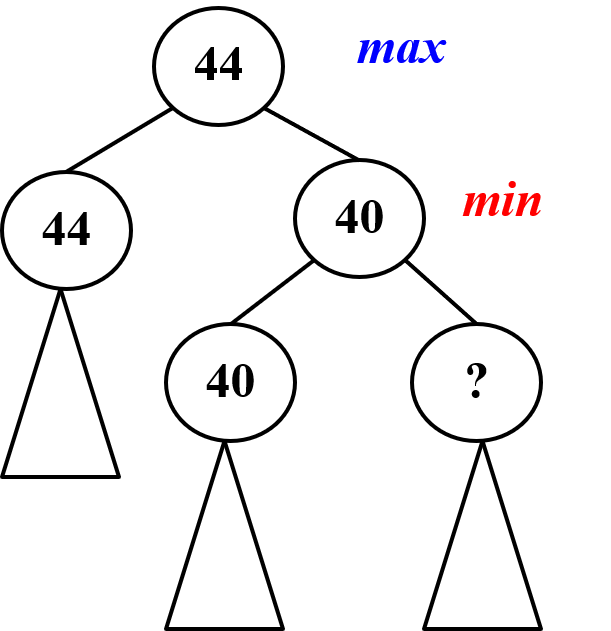
\includegraphics[width=\textwidth]{ADS6/a pruning}
        \caption{$\alpha$ pruning}
    \end{subfigure}
    \begin{subfigure}{0.16\textwidth}
        \centering
        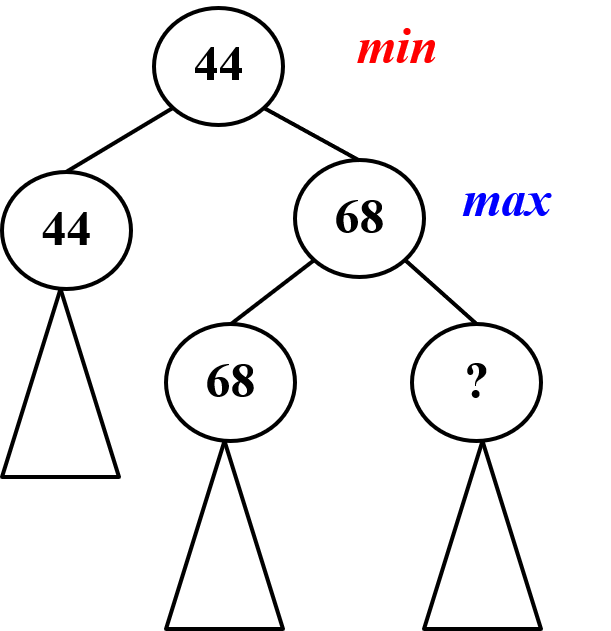
\includegraphics[width=\textwidth]{ADS6/b pruning}
        \caption{$\beta$ pruning}
    \end{subfigure}
    \caption{$\alpha$-$\beta$ pruning}
\end{figure}

When both techniques are combined.  In practice, it limits the searching to only $O(\sqrt{N})$ nodes, where $N$ is the size of the full game tree.




